\documentclass[conference]{IEEEtran}
\usepackage{cite}
\usepackage{amsmath,amssymb,amsfonts}
\usepackage{algorithmic}
\usepackage{graphicx}
\usepackage{textcomp}
\usepackage{xcolor}
\usepackage{pgfplots}
\pgfplotsset{compat=1.18}

% Use Times-like font with full Unicode and bold support
\usepackage{newtxtext,newtxmath}

\usepackage{tikz}
\usetikzlibrary{arrows.meta, positioning, shapes.geometric}
\usepackage{pagecolor}

% add for full-width equations in two-column layout
\usepackage{cuted}      % provides strip environment for full-width equations
\usepackage{stfloats}   % improved placement for figure*/table* floats

\usepackage{booktabs}
\usepackage{makecell}

% Hyperref package for PDF bookmarks and outlines
\usepackage[bookmarks=true,
            bookmarksnumbered=true,
            bookmarksopen=true,
            bookmarksopenlevel=2,
            pdfborder={0 0 0},
            pdfstartview=FitH,
            pdftitle={The Calçotada Protocol: Equity Peg Tokens for Decentralized Venture Capital},
            pdfauthor={Dr. Julià Delos Ayllón},
            pdfsubject={Blockchain-based Venture Capital Protocol},
            pdfkeywords={Blockchain, Venture Capital, Decentralized Finance, Tokenization, Equity Peg Token, DAO},
            colorlinks=true,
            linkcolor=black,
            citecolor=black,
            urlcolor=blue,
            filecolor=black]{hyperref}

\usepackage{bookmark} % Enhanced bookmark handling
\usepackage{microtype}
\usepackage{xurl}
\usepackage{hyperref}
\usepackage{tabularx}

\setlength{\emergencystretch}{3em}
\sloppy

% Define a very gentle pastel green for the background
\definecolor{gentlegreen}{RGB}{245, 252, 245}
\pagecolor{gentlegreen}
\begin{document}

% Force page numbers to appear
\thispagestyle{plain}
\pagestyle{plain}

\title{The Calçotada Protocol: \ Equity PEG Tokens for Decentralized Venture Capital}

\author{\IEEEauthorblockN{Dr. Julià Delos Ayllón}
\IEEEauthorblockA{\textit{The Calçotada Company} \\
Eindhoven, Netherlands \\
ceba.contract@lacalcotada.com}}

\maketitle
\thispagestyle{plain} % Ensure page number on first page

\begin{abstract}
The Calçotada Protocol turns seed capital—high-return Real World Assets traditionally reserved for venture capitalists—into performance-pegged tokens called Performance Equity Growth (PEG) tokens. These tokens track company valuation milestones and feature protocol-enforced buybacks inspired by a convertible note, using a Dynamic Convertibility Condition (DCC) method to enable buybacks outside a larger sale. This gives retail investors structured exposure to the same upside potential that drives early-stage funding rounds.

This document presents an early MVP implementation and lays the foundation for a broader, community-driven protocol. We invite collaborators—from financial engineers to DAO architects—to help shape this emerging standard and support its development through grants and other contributions. By channeling speculative energy toward real company growth, the Calçotada Protocol—named after the Catalan communal food feast—creates a new class of venture-backed assets and opens a powerful funding channel for traditional startups outside the crypto-native sphere.
\end{abstract}
\vspace{1em}

\begin{IEEEkeywords}
Blockchain, Venture Capital, Real World Assets (RWAs), Performance-Pegged Tokens (PEGs), Tokenized Private Equity, Startup Funding, Retail Investing, Protocol-Enforced Buybacks, Decentralized Autonomous Organization (DAO), Open Protocol
\end{IEEEkeywords}

\section{Introduction: A Foundation for Real-World Crypto Value}

While blockchain has the potential to transform financial systems, a significant portion of the crypto landscape is dominated by speculative, zero-utility assets that contribute little to real economic value. This creates a cycle of hype and volatility that undermines trust in Web3's promise as a foundation for meaningful innovation. At the same time, traditional venture capital remains a centralized and exclusive industry, leaving many high-potential founders without access to early-stage capital.

The \textbf{Calçotada Protocol}—the official proposal by The Calçotada Company to raise its seed round—proposes a new, community-driven path by introducing a class of Performance Equity Growth (PEG) tokens. These tokens bridge the gap between speculative crypto capital and real-world company growth by aligning token value directly with company success. PEG tokens are issued against company valuation milestones and are governed by smart contracts that enforce financial transparency and buyback mechanisms. Inspired by convertible notes, the protocol uses a \textbf{Dynamic Convertibility Condition (DCC) method} to enable buybacks outside of a traditional exit event, providing retail investors with structured exposure to the same upside potential that drives early-stage funding rounds.

This paper presents the protocol as both a Minimum Viable Product (MVP) and an open specification. By defining a transparent, programmable approach to seed funding, it challenges the concentration of venture power and expands access to capital for a more diverse range of founders. Our work directly addresses the limitations of existing token-based financing models, which often lack a strict link between token value and company performance. It transforms speculation into structured investment, paving the way for a more robust and inclusive economic system built on blockchain infrastructure.

\subsection{Protocol Development Anchored in Real Operations}

Critically, the Calçotada Protocol is not merely theoretical. Its initial development is directly anchored in the funding needs of a functioning startup: \textit{The Calçotada Company}, a food-tech venture with a validated business model and operational roadmap. By designing the protocol alongside an active business, its architecture, incentives, and smart contracts are built in response to actual operational constraints—not abstract scenarios.

This parallel development places The Calçotada Company in a unique position as a test bench for Web3 integration. The startup can experiment with blockchain-based governance, tokenized financial flows, and smart contract logic, while simultaneously exploring applications within traditional operations, such as e-commerce and app development. This applied approach enables rigorous testing of buyback mechanisms, community governance, and financial interactions in a live environment, creating a higher-trust, more credible foundation for both the company and the broader protocol rollout.

---

\section{State of the Art: The Problem of Disconnected Capital}

The promise of blockchain is often met with the reality of disconnected capital. On one side, startups—especially those with real-world products—face a significant challenge in raising seed capital. Traditional venture capital is a centralized system that often overlooks founders outside of its established networks, creating a \textbf{funding gap} for a diverse range of innovative ideas. The well-known "tunnel vision" associated with centralized VC is discussed in the first chapter of \textit{Power and Progress} (2023) by Acemoglu and Johnson \cite{acemoglu2023power}, where they argue that innovation is not a neutral force but often serves the narrow agendas of those who control capital flows. This dynamic is amplified by the structure of the VC industry, which filters startup potential through a small number of high-net-worth individuals and institutions, leading to centralized decision-making and trend-following capital allocation.

This challenge is also implicitly supported by research from Headd (2003) \cite{headd2003redefining}, which notes that businesses with more resources and better financing have a higher chance of survival, and by Henrikson et al. (2010) \cite{henrikson2010funding}, which, while challenging the concept of a "static" funding gap, highlights that a lack of resources remains a central issue for entrepreneurs at the early stages of a new venture.

On the other side, the crypto market is flooded with massive amounts of retail investment. However, this capital is largely funneled into speculative ventures like meme coins and highly volatile altcoins, creating a cycle of pump-and-dump schemes with no connection to real-world value creation. While often dismissed as irrational, these investors are simply seeking accessible, high-risk, high-return opportunities that are unavailable in traditional markets.

The Calçotada Protocol is designed to bridge the gap between traditional venture capital and decentralized finance. It aims to redirect retail crypto investment from speculative assets to tangible innovation by creating a new, inclusive form of venture funding.

\subsection{The Rise—and Limits—of Token-Based Startup Financing}
Blockchain-based financing emerged as a promising alternative to VC dominance. ICOs, in particular, were initially seen as a democratized fundraising mechanism. However, studies such as Howell et al. (2020)~\cite{howell2020initial} and Catalini \& Gans (2019)~\cite{catalini2019some} found that token value in these offerings was often driven by speculative market sentiment rather than by startup fundamentals. The lack of intrinsic utility or rights backing these tokens made them volatile and prone to pump-and-dump cycles.

Attempts to bridge token value with financial fundamentals include models like the Simple Agreement for Future Tokens (SAFT), token warrants~\cite{lw2019token}, and hybrid governance protocols (e.g., Compound, MakerDAO). Yet these models stop short of enforcing a valuation peg—a strict, transparent link between company performance and token economics.

Moreover, the majority of these fundraising models have been designed to serve crypto-native projects—protocols, DeFi platforms, and dApps—rather than general startups with traditional product-market strategies or offline operations. This creates a structural exclusion: while crypto capital is abundant, it remains inaccessible to founders outside the ecosystem who lack deep technical ties to Web3 culture or tooling.

As blockchain infrastructure matures and regulatory clarity improves, there is a growing opportunity to extend DAO-based venture financing to traditional startups. Doing so requires token models that reflect the financial logic of early-stage equity, not speculative or utility-only design.

\subsection{The Missing Piece: Equity Peg Tokens}

Recent research by Cao (2023)~\cite{cao2023token} differentiates between token and equity-based startup financing, concluding that token sales provide liquidity but introduce misalignment risks unless structured to reflect startup success metrics. This gap motivates the core innovation of the Calçotada Protocol: the design of Performance Equity Growth (PEG) tokens, which are governed by on-chain logic tied to company valuation.

PEG tokens act as a synthetic representation of equity performance—without requiring the legal complexity of security issuance—by enforcing treasury-backed buyback mechanics once valuation milestones are achieved. This model builds on the foundations of tokenized convertible instruments but extends them with financial enforcement via smart contracts, oracle-fed financial data, and protocol-level transparency. Research by J.P. Morgan (2025)~\cite{bain2023tokenization} further highlights the potential for tokenization to democratize access to illiquid private assets for individuals.

PEG tokens aim to serve not only crypto-native ventures but any startup that can benefit from structured capital, community engagement, and transparent governance. This extends the reach of token-based financing beyond the narrow corridor of Web3-native businesses and opens the door for new industries to access decentralized capital infrastructure.

\subsection{Beyond Speculation: Capturing Retail Energy for Innovation}

Another key motivation for this protocol is the observed misalignment between retail investor behavior and long-term innovation. Meme coins and speculative tokens have attracted vast inflows from non-accredited investors who are excluded from traditional VC. While often dismissed as irrational actors, these users are expressing a real hunger for high-upside opportunities.

Recent studies highlight that meme coins (e.g., Dogecoin, Shiba Inu, PEPE, and \$TRUMP) are driven primarily by social momentum, narrative virality, and celebrity or influencer activity rather than utility or project fundamentals \cite{rutgers2023meme, sSrn4891841}. Despite high volatility, they consistently attract hundreds of thousands of wallets, as seen in the over 700,000 wallets impacted by the \$TRUMP crash in 2024 \cite{wikipediaTrump}.

Far from being irrational, these users are seeking accessible, high-upside entry points—currently unavailable through traditional equity mechanisms. As retail sentiment continues to move faster than institutional cycles, it represents a powerful force if properly directed \cite{marketwatch2022retail, arxiv2104.01847}.

Redirecting this energy from pure speculation toward structured, valuation-pegged startup exposure could unlock meaningful capital for undeserved founders. In this sense, \textbf{PEG tokens} are not just technical artifacts—they are social and economical instruments. They challenge the concentration of venture power, expand the set of founders with access to capital, and provide retail investors with an opportunity to participate in shaping the economic frontier.

\section{Fundamentals of the Calçotada Protocol}

The protocol's core contribution is a compact, auditable set of financial equations that define tokenomics with the same economic logic used in seed‑stage VC deals. These equations—implemented as smart‑contract primitives combining SAFE‑style parameters, bonding‑curve minting and valuation‑anchored buyback pricing—create a synthetic, traceable mapping between company performance and per‑token economic value. The design therefore delivers two complementary upsides for token holders: (1) an equity‑like return profile driven by realized and projected company value, and (2) on‑chain liquidity through protocol‑enforced buybacks and treasury mechanisms. By encoding these relationships deterministically on‑chain, the protocol makes the link between corporate value creation and token market behavior transparent, auditable and governable by the DAO.

Key elements include a dual‑token architecture (NFTs for governance and rights; RMSC for financial exposure), capital‑backed minting (tokens minted only when new capital is contributed), protocol‑enforced buybacks that provide on‑chain liquidity and a valuation‑anchored floor, DAO governance over treasury reuse and secondary issuances, and auditable on‑chain accounting of supply and reserves.

This overview focuses on the protocol’s intent: to automate a decentralized VC primitive that issues equity‑like tokens, enforces transparent economic rules, and provides market liquidity for retail participants.

\subsection{Dual-Token Issuance and Deflationary System}

The protocol uses a dual-token model, where token issuance reflects real capital added to the company. Both tokens have a \textbf{strictly capped supply} corresponding to the target raise.

\begin{itemize}
    \item \textbf{CalcotCoin (NFT):} Serves as a founding membership, granting governance rights, access to exclusive company benefits, and priority eligibility for buybacks. NFTs are released in \textbf{batches}, each associated with a round of capital addition. Purchasing an NFT is equivalent to joining as a founding investor. The NFT itself does not guarantee a fixed ROI; its value comes from the combination of benefits, governance privileges, and buyback access.

    \item \textbf{Romesco (RMSC) Token:} A fungible token reflecting the company’s Performance Equity Growth (\textbf{PEG}) value. RMSC tokens are allocated to participants based on their capital contribution, providing financial exposure to the company’s performance. Supply is capped by the total target raise, ensuring tokens are only minted when new capital enters the system.
\end{itemize}

\subsection{Participation and Token Allocation}
Capital additions are issued in \textbf{batches}. In each batch, the price of participation increases, reflecting the added value and risk for early investors.

Participation proceeds through clearly defined steps:

\begin{enumerate}
    \item \textbf{Capital Contribution:} The participant provides capital to join a funding batch.
    \item \textbf{RMSC Minting:} The contributed capital is converted into newly minted RMSC tokens according to a predefined price bonding curve.
    \item \textbf{RMSC Allocation:}
    \begin{itemize}
        \item \textbf{50\% to Company Treasury:} These tokens serve as RMSC reserves, securing governance and buyback privileges via the NFT.
        \item \textbf{50\% to Participant:} Retained as a participation bonus, giving direct financial exposure to the company's growth.
    \end{itemize}
    \item \textbf{NFT Issuance:} In exchange for the treasury allocation, the participant receives a founding NFT, granting governance rights, community access, and buyback eligibility.
\end{enumerate}

\begin{figure}[ht]
\centering
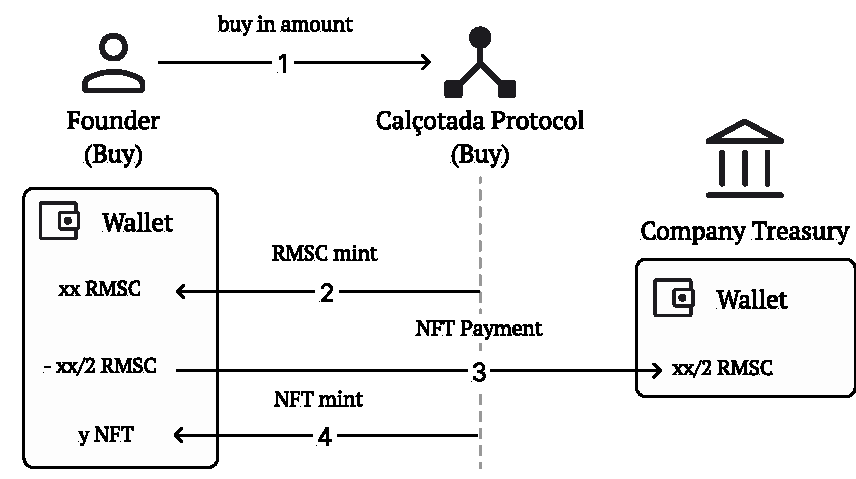
\includegraphics[width=0.45\textwidth]{minting-diagram.pdf}
\caption{Token minting process sequence diagram}
\label{fig:minting-strategy}
\end{figure}

In parallel, there is a \textbf{free pool of RMSC tokens} for participants seeking larger financial exposure beyond the batched issuances.

This mechanism ensures that \textbf{RMSC supply grows strictly in proportion to capital raised}, maintaining a transparent and auditable tokenomics framework. Simultaneously, the \textbf{NFT layer anchors governance, community access, and buyback privileges}, while RMSC serves as the liquid instrument for financial participation.

\subsection{RMSC Treasury and Its Role}

Half of the RMSC tokens minted through NFT purchases are transferred to the \textbf{company treasury} as reserves. This treasury has a strategic purpose:

\begin{itemize}
    \item \textbf{Liquidity Provision:} A portion of the treasury can be deployed in liquidity pools to support RMSC market activity without increasing total supply.
    \item \textbf{Airdrops:} The treasury can distribute RMSC to NFT holders as rewards or incentives, strengthening community engagement.
    \item \textbf{Growth Initiatives:} The treasury provides capital for strategic programs and partnerships, enabling the company to expand its ecosystem while preserving token scarcity.
\end{itemize}

By maintaining these reserves, the treasury allows the company to execute financial strategies and community programs \textbf{without affecting the capped total supply of RMSC}, ensuring transparency and long-term sustainability of the tokenomics framework.

% Inserted explanatory subsection:
\subsection{Buybacks, Treasury Reuse, and the Growth Cycle}

Buybacks executed by the company remove RMSC from active circulation (either by on‑chain burn or by transferring tokens into a non‑circulating treasury lock). Removing tokens from circulation tightens the available float and, all else equal, increases the economic value per remaining token. This deflationary action, when paired with valuation‑based buyback pricing, establishes a transparent floor and creates upward pressure on market prices during execution.

Treasury‑held RMSC are an economic asset of the company. With explicit DAO approval and governance controls, these treasury tokens can be re‑deployed as a form of capital raising—sold in controlled secondary issuances or used in strategic financing rounds similar to follow‑on series. Such reuse effectively converts treasury holdings back into operating capital, but it increases circulating supply and can be dilutive unless offset by concurrent buybacks or demonstrable value accretion from the invested proceeds.

Crucially, reinvesting proceeds into productive company growth is the mechanism that improves underlying valuation. Higher realized profits, margin expansion, or successful scaling raise the on‑chain DCF valuation, which in turn increases the buyback multipliers ($Tk_{ROI}$) used to price future buybacks. In this way the protocol creates a virtuous cycle: disciplined reinvestment raises company value, which raises the valuation anchor for RMSC, which benefits holders when buybacks are executed.

To preserve transparency and guard against circular financing, the protocol must codify:
\begin{itemize}
    \item whether repurchased tokens are burned or retained in treasury (and the conditions for each),
    \item governance thresholds and quorum for any treasury resale or secondary issuance,
    \item on‑chain reporting of totalSupply, circulatingSupply, treasuryBalance, and retiredSupply, and
    \item limits and execution mechanisms for buybacks  to reduce market impact and front‑running risk.
\end{itemize}

Finally, tokenization primarily adds liquidity: it provides an on‑chain exit path for investors who wish to realize value prior to a traditional liquidity event. That liquidity—backed by treasury reserves, valuation‑anchored buybacks, and transparent on‑chain accounting—improves price discovery and investor confidence while retaining the company’s ability to deploy capital strategically under DAO oversight.
%
\subsection{Valuation Methodology}
Startup valuation is inherently challenging due to limited historical data, high uncertainty in cash flows, and rapidly evolving market conditions. Nevertheless, academic research and industry practice support the use of Discounted Cash Flow (DCF) as a rigorous, theoretically grounded approach for estimating firm value, even in early-stage ventures \cite{Laitinen2019,Olsen2019,Arefmanesh2025,Montani2020,Steiger2010}. The DCF methodology provides a transparent, auditable framework that reflects the time value of money and the risk-adjusted potential of future cash flows.

To provide a verifiable and auditable valuation, the protocol proposes a hybrid approach that leverages both a deterministic on-chain model and the potential for a traditional market exit:

\begin{itemize}
\item \textbf{Dynamic On-Chain Discounted Cash Flow (DCF):}
The primary valuation method is an on-chain DCF model that can be updated with actual operational data. Instead of relying solely on projected cash flows, past periods are replaced with real company performance metrics, including revenues, costs, margins, and CAPEX. This allows the protocol to calculate a near real-time company valuation ($V_\text{daily}$), bridging traditional DCF theory with dynamic operational insight. By executing the inputs and calculations within smart contracts, the valuation remains tamper-proof, fully transparent, and accessible to all token holders \cite{Laitinen2019,Steiger2010}.

\begin{equation}
V_{\text{daily}} = \sum_{t=0}^{T} \frac{\text{FCF}{t,\text{actual}}}{(1+r)^t} + \sum{t=T+1}^{\infty} \frac{\text{FCF}_{t,\text{projected}}}{(1+r)^t}
\end{equation}


\item \textbf{Open Market Exit:}
In the event of a traditional liquidity event (e.g., acquisition or Initial Public Offering), the protocol's valuation is superseded by the actual market valuation. This ensures that token holders are aligned with real-world outcomes and can benefit from successful exits, complementing the deterministic DCF framework \cite{Montani2020,Olsen2019}.
\end{itemize}

\subsection{The Buyback Mechanism}

The buyback mechanism is the core instrument of the tokenomics, controlling both the market supply and the liquidity pool of RMSC tokens. It provides a transparent, decentralized exit route for token holders while preserving company flexibility in valuation and capital management.

The deterministic Token ROI (\(\mathrm{Tk_{ROI}}\)) is computed using the adjusted company valuation and a formal SAFE (Simple Agreement for Future Equity) framework. Unlike traditional SAFEs, the purpose here is not direct equity conversion, but to anchor RMSC token liquidity and enforce price discipline in the open market.

The SAFE-based buyback mechanism is formally defined by four parameters:

\begin{itemize}
    \item \textbf{Discount Rate (\(d\))} – reduces the effective valuation for early token holders, providing an incentive for early participation.
    \item \textbf{Valuation Cap (\(V_\text{cap}\))} – the maximum valuation used in calculating ROI, protecting token holders from excessive dilution.
    \item \textbf{Interest Rate (\(i\))} – a simple accrual representing the time-based value until buyback or conversion.
    \item \textbf{Years (\(year\))} – the time period over which the interest accrues, typically aligned with the expected duration until a liquidity event.
\end{itemize}

Formally, the Token ROI is computed as:

\begin{equation}
\mathrm{Tk_{ROI}} = \max\Big[   \frac{ (1 + i)^{year}}{ (1 - d)}  , \frac{ V_\text{cap}}{V_\text{on-chain}} \Big]
\end{equation}
where:

\begin{itemize}
    \item \(V_\text{valuation}\) is either the on-chain DCF valuation (\(V_\text{on-chain}\)) or market exit valuation (\(V_\text{market}\)).
    \item \(\overline{P}_\text{mint}\) is the average mint price of the RMSC of the overall minted supply.
\end{itemize}

The final per-token buyback price is:

\begin{equation}
P_\text{buyback} = \mathrm{Tk_{ROI}} \times \overline{P}_\text{mint}
\end{equation}

The execution of buybacks is subject to the company's treasury liquidity and governance oversight.

This buyback mechanism is instrumental in making the tokenomics work by controlling the market supply and liquidity pool of RMSC. It leverages the SAFE framework to allow flexible company valuation and price discovery, benefiting both the company and token holders. Importantly, the mechanism does not directly convert tokens into company equity; instead, it ensures liquidity exists that influences the RMSC token price in the open market.

\section{Protocol MVP Implementation}

\usetikzlibrary{arrows.meta, positioning, shapes.geometric}

\begin{figure}[ht]
\centering
\scalebox{0.5}{%
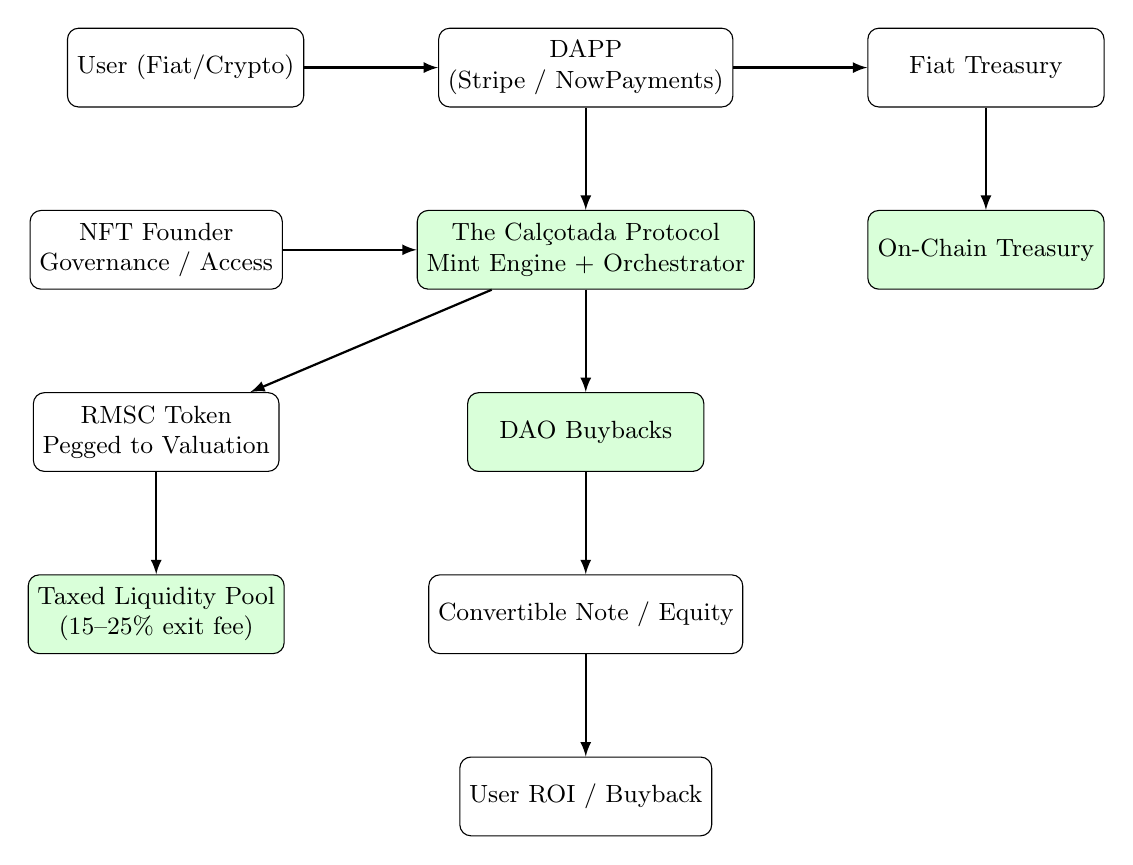
\begin{tikzpicture}[node distance=1.3cm and 1.7cm, every node/.style={font=\small}]

% Styles
\tikzstyle{box} = [draw, rounded corners, align=center, minimum width=3cm, minimum height=1cm, fill=white]
\tikzstyle{greenbox} = [box, fill=green!15]
\tikzstyle{arrow} = [->, thick, >=latex]

% Nodes
\node[box] (user) {User (Fiat/Crypto)};
\node[box, right=of user] (dapp) {DAPP\\(Stripe / NowPayments)};
\node[box, right=of dapp] (fiat) {Fiat Treasury};
\node[greenbox, below=of fiat] (onchain) {On-Chain Treasury};

\node[greenbox, below=of dapp] (protocol) {The Calçotada Protocol\\Mint Engine + Orchestrator};

\node[box, left=of protocol] (nft) {NFT Founder\\Governance / Access};
\node[box, below=of nft] (rmsc) {RMSC Token\\Pegged to Valuation};

\node[greenbox, below=of protocol] (dao) {DAO Buybacks};
\node[box, below=of dao] (equity) {Convertible Note / Equity};
\node[box, below=of equity] (payback) {User ROI / Buyback};

\node[greenbox, below=of rmsc] (tlp) {Taxed Liquidity Pool\\(15–25\% exit fee)};

% Arrows
\draw[arrow] (user) -- (dapp);
\draw[arrow] (dapp) -- (fiat);
\draw[arrow] (fiat) -- (onchain);
\draw[arrow] (dapp) -- (protocol);

\draw[arrow] (nft) -- (protocol);
\draw[arrow] (protocol) -- (rmsc);
\draw[arrow] (protocol) -- (dao);
\draw[arrow] (dao) -- (equity);
\draw[arrow] (equity) -- (payback);
\draw[arrow] (rmsc) -- (tlp);

\end{tikzpicture}%
}%
\caption{Simplified architecture of the Calçotada Protocol: dual-token issuance and treasury-integrated valuation peg.}
\end{figure}


 The architecture consists of four core smart contracts that work in concert: CalcotCoin (NFT), Romesco (RMSC token), Calçotada (orchestrator), and NormalizeToEuro (oracle integration). 

\subsection{CalcotCoin NFT: Governance and Foundational Access}

\begin{figure}[ht]
\centering

\includegraphics[width=0.3\textwidth]{calcot-coin-logo.png}
\caption{Calçot-Coin (CEBA) - The NFT representing community participation and governance}
\label{fig:calcotcoin-logo}
\end{figure}

The \textit{CalcotCoin} (CEBA) contract implements an ERC721 NFT system designed to recognize early supporters and provide governance rights. The current implementation features:

\textbf{Technical Specifications:}
\begin{itemize}
    \item Token Type: NFT (ERC721)
    \item Token Name: Calçot-Coin
    \item Token Symbol: CEBA
    \item Batch: 0 (Genesis)
    \item Fixed supply of 333 NFTs (CEBA Genesis edition)
    \item Public allocation: 300 NFTs
    \item Pre-mint - Reserved Treasury: 33 NFTs
    \item Linear pricing mechanism from 0.4€ to 0.5€ RMSC per NFT
    \item Buy in price: €100 
    \item One vote per wallet 
\end{itemize}


\subsection{RMSC Token: Equity-Pegged Financial Instrument}

\begin{figure}[ht]
\centering

\includegraphics[width=0.3\textwidth]{rmsc_logo.png}
\caption{Romesco (RMSCU) - The fungible token representing the "secret sauce" of venture returns}
\label{fig:rmsc-logo}
\end{figure}

The \textit{Romesco Token (RMSC)} is the core financial instrument of the protocol, implemented as an ERC20 token with ERC1363 and ERC20Permit extensions for enhanced functionality.

\textbf{Technical Implementation:}
\begin{itemize}
    \item Token Type: FT (ERC20)
    \item Token Name: Romesco
    \item Token Symbol: RMSCU
    \item Fixed maximum supply of 5,000,000 RMSC (hard cap enforced in contract)
    \item Premint Treasury: 200,000 RMSC for liquidity and operational needs
    \item $\boldsymbol{\overline{P}_\textbf{mint}}$: €0.557 per RMSC
    \item Pausable functionality for emergency situations
    \item Permit functionality for gasless approvals
    \item ERC1363 support for single-transaction transfers and callbacks
\end{itemize}

\textbf{Economic Design:}
\begin{itemize}
    \item Minting controlled by the orchestrator contract only
    \item No burn functionality for regular users (maintains supply integrity)
    \item Designed for future buyback mechanism at €1.5–€3.0 per RMSC
    \item Starting valuation implies approximately €0.40–€0.70 per RMSC
\end{itemize}


\subsection{Calçotada Orchestrator: Protocol Coordination}

The \textit{Calçotada} contract serves as the central orchestrator, coordinating interactions between all protocol components:

\textbf{Core Functions:}
\begin{itemize}
    \item Manages the dual-minting mechanism for NFT purchases
    \item Controls RMSC minting according to bonding curve pricing
    \item Handles both public and private sale mechanisms
    \item Integrates with NormalizeToEuro for multi-currency support
\end{itemize}

\textbf{Bonding Curve Implementation:}
The orchestrator implements a normalized bonding curve using:
\begin{itemize}
    \item Q16.16 fixed-point arithmetic for precision
    \item Configurable sigmoid curve shape for optimal price discovery
    \item Integration with trapezoidal rule for accurate pricing
    \item Starting price: €0.40 per RMSC, ending price: €0.70 per RMSC
\end{itemize}

\textbf{Transaction Fee Structure:}
\begin{itemize}
    \item NFT purchases: €4.50 transaction fee
    \item RMSC purchases: €2.50 transaction fee
\end{itemize}

\subsection{Price Oracle Integration}

The \textit{NormalizeToEuro} contract provides real-time price conversion using Chainlink oracles:

\textbf{Oracle Feeds:}
\begin{itemize}
    \item ETH/USD, EUR/USD, and POL/USD price feeds
    \item Automatic conversion between EUR pricing and POL payments
    \item 18-decimal precision for all calculations
\end{itemize}

\subsection{Initial Supply and Distribution}

The initial supply of RMSC tokens is allocated in a controlled and transparent manner to recognize pre-protocol contributions and prepare for public issuance. No tokens are minted speculatively or granted without capital justification.

\subsubsection{Angel Investor Allocation}

Prior to the protocol's launch, a group of early angel investors provided capital to The Calçotada Company under a convertible loan agreement. These early backers are entitled to receive RMSC tokens at the protocol’s base issuance price, plus an interest premium to account for the time value of their risk.

\begin{itemize}
    \item \textbf{Base Price Conversion:} Angel investments are converted into RMSC at the same base price offered during the initial public issuance phase.
    \item \textbf{Interest Adjustment:} A fixed 7\% interest rate is applied to the original invested amount, and this adjusted total determines the corresponding RMSC allocation.
    \item \textbf{Non-inflationary Grant:} These tokens are accounted for as part of the protocol's total capped supply and are not created in excess of the 5 million RMSC ceiling.
\end{itemize}

\subsubsection{Pre-Mint Reserve}

In addition to angel investor conversion, a total of 200,000 RMSC tokens are pre-minted and held in the protocol treasury for operational, liquidity, and market stabilization purposes. 

\subsection{Public Issuance}

All remaining RMSC tokens are made available through direct, capital-backed purchase via Web3 interface.
\subsection{Planned Participation Batches and RMSC Minting}
The current minting strategy involves multiple participation batches, each with distinct NFT offerings and associated RMSC minting. As described in the following table, each batch has specific parameters for NFT supply, buy-in price, and RMSC allocation.

\begin{table}[ht]
    \centering
    % This command makes the multi-line headers bold and centered
    \renewcommand{\theadalign}{bc}
    \caption{NFT Batches and Associated RMSC Minting}
    \label{tab:nft_batches}
    \begin{tabular}{@{}lcccc@{}}
        \toprule
        % Use \thead to create multi-line headers that fit the column
        \thead{Batch} & \thead{NFT \\ supply} & \thead{Buy-In \\ price (€)} & \thead{$\boldsymbol{\overline{P}_\textbf{mint}}$ \\ (€)} & \thead{RMSC \\ supply} \\
        \midrule
        Calçot Coins  (MVP) & 333   & 100   & 0.45  & 74,000    \\
        \midrule 
        FounderPass 1 & 1111   & 125   & 0.50  & 277,750   \\
        FounderPass 2 & 1111  & 250   & 0.525 & 529,000   \\
        FounderPass 3 & 1111  & 375   & 0.55  & 757,000   \\
        FounderPass 4 & 1111  & 500   & 0.575 & 966,000   \\
        FounderPass 5 & 1111  & 625   & 0.60  & 1,157,000 \\
        \midrule
        \multicolumn{5}{c}{\textbf{Total: 5,888 NFTs}} \\
        \multicolumn{5}{c}{\textbf{2,047,025 € raised, 3,761,676 RMSC minted}} \\
        \bottomrule
    \end{tabular}
\end{table}


\subsubsection{Public RMSC Issuance via Bonding Curve}

The Calçotada orchestrator implements a sophisticated bonding curve mechanism for public RMSC sales:

\textbf{Technical Implementation:}
\begin{itemize}
    \item Normalized sigmoid curve stored as Q16.16 fixed-point values
    \item Configurable curve shape via uploadable parameters
    \item 16-step trapezoidal integration for accurate pricing
    \item Real-time POL/EUR conversion via Chainlink oracles
\end{itemize}


\begin{figure}[ht]
\centering
\begin{tikzpicture}
\begin{axis}[
    width=\linewidth,
    height=6cm,
    grid=both,
    xlabel={\textbf{Fraction of Supply Minted}},
    ylabel={\textbf{RMSC Price (€)}},
    title={Sigmoid Bonding Curve for Public RMSC Issuance},
    ymin=39, ymax=61,
    xmin=0, xmax=1,
    thick
]
\addplot[
    color=blue,
    mark=none
]
table[
    col sep=comma,
    x=fraction_minted,
    y=rmsc_price_eur
] {rmsc_sigmoid_curve.csv};
\end{axis}
\end{tikzpicture}
\caption{Sigmoid bonding curve used for public RMSC issuance pricing.}
\label{fig:sigmoidcurve}
\end{figure}


This curve allows early public buyers enjoy lower prices, and late-stage buyers pay a premium as the available supply nears exhaustion representing the less exposed risk.

\subsection{Network Deployment}
Polygon is selected as the base network for its:
\begin{itemize}
    \item Low transaction fees and fast confirmation times,
    \item Proven security track record via Ethereum finality,
    \item Established ecosystem of NFT and DeFi projects.
\end{itemize}

Deploying on Polygon enables frictionless user participation while ensuring composability with future liquidity protocols and DAO tools.

\section{Vision: From Meme Coins to PEG Coins}

This whitepaper presents not just a protocol implementation, but a vision for transforming venture capital through blockchain technology. We invite builders, researchers, and visionaries to join us in developing the foundational components for true DAO-based venture capital.

\subsection{Redefining PEG: From Price Stability to Performance Growth}

The term "PEG" in traditional crypto contexts typically refers to price-pegged assets like stable coins. We intentionally reappropriating this term to create a powerful contrast with MEME coins. While MEME coins represent pure speculation without underlying value, PEG (Performance Equity Growth) tokens represent the opposite: real value creation tied to company performance.

\textbf{The MEME vs PEG Paradigm:}
\begin{itemize}
    \item \textbf{MEME}: Speculation, hype-driven, no intrinsic value
    \item \textbf{PEG}: Performance-driven, value-backed, growth-oriented
\end{itemize}

Unlike traditional price pegs that maintain stable values, our PEG tokens are \textit{pegged to company growth}. This represents a new category of crypto assets:
\begin{itemize}
    \item Not pegged to a stable price (like USDT to USD)
    \item Not pegged to another asset (like WBTC to BTC)
    \item But pegged to a company's valuation trajectory and success
\end{itemize}

This redefinition serves a dual purpose: it creates a memorable contrast with MEME coins while accurately describing tokens that track real business performance. PEG tokens offer the excitement of venture returns with the substance of equity participation—transforming speculation into investment.


\section{Call for Builders and Contributors}

This whitepaper is a proposal and invitation. We seek:
\begin{itemize}
    \item \textbf{Protocol Developers:} To build standardized components
    \item \textbf{Oracle Integrators:} To validate fiat transactions
    \item \textbf{Financial Engineers:} To refine DCF models
    \item \textbf{Legal Experts:} To navigate regulatory frameworks
    \item \textbf{Community Leaders:} To educate and onboard users
    \item \textbf{Startup Founders:} To adopt and test the protocol
\end{itemize}

Many questions remain unanswered—optimal update frequencies, discount rates for pre-revenue startups, governance structures. These will be defined collectively as we build this new foundation for venture capital.

The Calçotada Protocol is more than technology; it's a movement toward democratized, transparent, and accessible startup funding. Join us in creating the future of venture capital.



\section{Team and Acknowledgments}

The Calçotada Protocol is driven by a dedicated team of RMSC holders representing the company's interests:

\textbf{Dr. Julià Delos Ayllón} - Founder and Chief Architect. With a distinguished career spanning from software to high-power systems, Dr. Ayllón holds a PhD in Electrical Engineering focused on power electronics and LED driver optimization. His professional journey includes roles at Philips Research, HP, and Lear Corporation, where he developed innovative solutions from embedded software to advanced power management systems. At Philips Research, he contributed to multiple patents in LED driver technology and integrated power systems. This deep technical expertise in hardware miniaturization and system optimization now informs his approach to blockchain protocol design. Dr. Ayllón founded The Calçotada Company with a vision to revolutionize access to food experiences through a Food Experience as a Service (FEaaS) business model—creating an "Airbnb for culinary experiences" that enables rapid scaling while preserving authentic local gastronomy. His unique background bridges hardware engineering, corporate R\&D, and entrepreneurial innovation, positioning him to architect protocols that merge real-world business models with decentralized finance.

\textbf{Dr. Louisa Spaans} - Medical doctor and protocol keyguard. Early angel investor and major RMSC holder safeguarding protocol integrity.

\textbf{Dr. Dimitri Pustakhod} - PhD and protocol keyguard. Strategic advisor and major RMSC holder ensuring governance alignment.

\textbf{Danail Hristov} - Telecom engineer and protocol keyguard. Technical advisor and major RMSC holder protecting protocol development.

This team represents the convergence of technical innovation, medical precision, business acumen, and entrepreneurial vision—united in democratizing access to venture capital through blockchain technology.

\section{Conclusion and Future Work}

The Calçotada Protocol represents a significant step toward democratizing venture capital through blockchain technology. By implementing tokenized convertible notes with clear valuation pegs, the protocol creates a bridge between traditional startup funding and decentralized finance.

\subsection{Current MVP Implementation}

The deployed Minimum Viable Product serves as a proof of concept and market validation tool:

\textbf{Implemented Features:}
\begin{itemize}
    \item Genesis collection of 333 CalçotCoin NFTs at €100 each
    \item RMSC token with 5M supply cap and bonding curve mechanics
    \item Dual-minting system rewarding early supporters
    \item Oracle integration for EUR/POL price conversion
    \item Basic treasury accumulation mechanism
\end{itemize}

\textbf{MVP Objectives:}
\begin{itemize}
    \item Demonstrate technical feasibility of tokenized venture funding
    \item Validate market demand with €30,000 initial raise target
    \item Build initial community of supporters and advisors
    \item Test smart contract security and gas efficiency
    \item Establish foundation for future protocol development
\end{itemize}

This MVP represents a testimonial to the work ahead, starting with a solid foundation of minting strategies and bonding curve sales mechanisms. The limited scope allows for careful iteration based on community feedback before expanding to the full protocol vision.


\section{The Calçotada Company: Protocol Sponsor}

\subsection{Company Overview}

The Calçotada Company is a Barcelona-based food-tech startup pioneering Food Experience as a Service (FEaaS). As the primary sponsor and first implementation of the Calçotada Protocol, the company serves as both a proof of concept and a real-world test case for tokenized venture funding.

\subsection{Business Model: FEaaS}

Food Experience as a Service (FEaaS) represents a paradigm shift in the hospitality industry:

\begin{itemize}
    \item \textbf{Scalable Culinary Experiences:} Transforming traditional dining into reproducible, high-quality experiences
    \item \textbf{Technology-Enabled Operations:} Leveraging automation and data analytics to optimize food service
    \item \textbf{Franchise-Ready Model:} Creating standardized processes that maintain authenticity while enabling rapid expansion
    \item \textbf{Cultural Preservation:} Protecting and promoting traditional Catalan cuisine through modern business practices
\end{itemize}

\subsection{Why Calçotada?}

The company takes its name from the traditional Catalan calçotada—a communal feast celebrating spring onions. This choice reflects:
\begin{itemize}
    \item Community-driven values aligned with DAO principles
    \item Scalable social experiences perfect for FEaaS model
    \item Strong cultural identity providing market differentiation
    \item Natural alignment between shared meals and shared ownership
\end{itemize}

\subsection{Protocol Synergy}

The Calçotada Company's use of the protocol demonstrates:
\begin{itemize}
    \item Real revenue generation for buyback mechanisms
    \item Clear valuation metrics through operational data
    \item Community engagement through product and investment
    \item Bridge between physical business and digital assets
\end{itemize}

\section{Cultural Inspiration: The Calçotada Tradition}

We'll be the first to admit it: a blockchain protocol named after a charred onion is unusual. But a \textit{calçot} is no ordinary onion. When grilled over an open flame, its outer layers burn away to reveal a heart of astonishingly sweet, tender deliciousness, perfect for dipping in a rich romesco sauce. The Calçotada Protocol draws its name from this Catalan tradition of \textit{la calçotada}, a communal feast that embodies shared effort and collective success—values we believe mirror our mission to democratize access to venture capital.

Beyond the symbolism, the names are a bit of fun that links the protocol directly to its sponsoring entity, \textbf{The Calçotada Company}. We believe that the success of our fundraising will bring us all a step closer to earning a seat at a real \textit{calçotada} feast. It's a culinary reward for a financial breakthrough.

The protocol's dual-token architecture reflects this heritage:
\begin{itemize}
    \item \textbf{The NFT (Calçot-Coin)}: Represents governance and participation. NFT holders are part of the decision-making collective, with voting rights and access to benefits as the company and protocol grow. This also guarantees participation in yearly meetings to try and enjoy the company’s products. The NFTs are freely tradable, and holders will have founding advantages in financing and the use of services.
    \item \textbf{The RMSC Token (Romesco)}: Represents capital and returns. The freely tradable RMSC token is designed to capture company performance while remaining detached from governance, preventing the concentration of influence among large holders. The secret, after all, is in the sauce.
\end{itemize}

Ultimately, retaining these names provides a distinctive, culturally resonant identity, reinforcing the connection between the protocol and The Calçotada Company, and ensuring brand consistency and long-term visibility.
\bibliographystyle{IEEEtran}
\bibliography{references}

\end{document}
